% Template for ICASSP-2020 paper; to be used with:
%          spconf.sty  - ICASSP/ICIP LaTeX style file, and
%          IEEEbib.bst - IEEE bibliography style file.
% --------------------------------------------------------------------------
\documentclass{article}
\usepackage{spconf,amsmath,graphicx}

% Example definitions.
% --------------------
\def\x{{\mathbf x}}
\def\L{{\cal L}}

% Title.
% ------
\title{IMPLEMENTING AN OBJECTIVE FUNCTION AND REPORTING THE EFFECTS OF REGULARISATION ON GENERATIVE MODELS}
%
% Single address.
% ---------------
\name{Chad Kakau \thanks{AIML425}}
\address{Victoria University, Wellington}
%
%
\begin{document}
%\ninept
%
\maketitle
%
\begin{abstract}
this paper revises the concept of objective functions as applied in machine learning and identifies the SELECTED OBJECTIVE FUNCTION used by the authors in the implementation of a generative neural network.  The generative model maps a gaussian distribution to a uniform distribution, then maps the uniform distribution to a gaussian distribution, for a concatenated gaussian to gaussian network.  This paper lists the three main objective functions used in neural networks and \bf{SOMETHING TO SAY GOES THROUGH THE MATH of the selected function:  .}  The results of the implemented neural network show that 
\end{abstract}
%
\begin{keywords}
One, two, three, four, five
\end{keywords}
%
\section{Introduction}
\label{sec:intro}
%
Neural networks have become a mainstay of image processing over the last two decades (compare \cite{parisi1998car} and \cite{naranjo2020review}) 

\section{Objective function}
\label{sec:format}

We train a neural network using stochastic gradient descent so that it can iteratively learn and adjust from the prediction (based on each instance, or input vector) and distance from the actual target (output vector).  One of the main decisions for the design of the network is the selection of an objective function to drive the model predictions toward the target.  Although numerous objective functions are possible, this implementation uses the Maximum Mean Discrepancy which measures the distance between two distributions.  For optimisation the model aims to minimise MMD.  Before working through the theory of the MMD, we need to first briefly discuss the kernel - a concept which has taken several days of bashing my head against the internet wall, for me to finally come to grips with.  

\subsection{The kernel function reduces the complexity of calculation without sacrificing detail}
\label{ssec:kernel}

After several lectures, reviews of lecturs, scanning of the internet and multiple re-visits to the wikipedia, I think the kernel, is a matrix that transforms our input vector in a lower dimensional space to the dot product output vector in a higher dimensional space \cite{wilimitis_2019} \cite{hofmann2008kernel}.  I struggled alot with the concept of the kernel, because I didn't take the time to look up what an inner product means... it turns out, an inner product is the result of multiplying two vectors and resolves to a scalar value.  

For instance, for the function $h(\cdot)$, in a reproducing kernel Hilbert space (I can't, so here is a link to an accessible explanation...), with kernel $k:$, then $h(x) =\langle k(x, \cdot ), h ( \cdot) \rangle$.

\subsection{Maximum Mean Distribution as the objective function}
\label{ssec:mmd}

With the distribution $p_Y$ as:  

$\frac {1}{n(n-1)}\sum_{i\ne j} k(y^{(i)}, y^{(j)})$  

and $p_X$ as:   

$\frac {1}{m(m-1)}\sum_{i\ne j} k(x^{(i)}, x^{(j)})$,  

where $k(x, y)$ is a positive definite kernel (in this case, the Gaussian
kernel 
$$
\begin {aligned}
MMD&(\{x^{(i)}\}_{i=1, ..., m}, \{y^{(j)}\}_{j=1, ..., n}) \\
  & = \\ 
  & + \\
  & - 2\frac{1}{mn}\sum_{i,j}k(x^{(i)},y^{(j)})
\end {aligned}
$$


%
\section{RESULTS}
\label{sec:results}
%
The results show that training a network to learn a Gaussian to Uniform distribution is fairly successful, evidenced by the similarity between the target data and the test data for the first part of the training.  Some of the learned network projects outside of the target area (i.e. greater than 1), which is likely an error in the transformation math (i.e. no epxlicit constraint placed on the output of the $f_1$ network.  Training the network from uniform to Gaussian was less successful, resulting in a skewed dataset with a high proportion of datapoints near the mean, but not is equally spread as the training data.  This is apparent in the training data being spread evenly across the two dimensions resulting in a circular distributin on the plot.
there is a difference between regularisation values at $L2 = {1e^{-6}, 1e^{-2}, 1}$, but it is diffiult to discern from the plots.  Best performance across both networks ($f_1$ an $f_{2a}$) was achieved with $L2 = 1e^{-6}$, followed by $L2 = 1e^{-2}$ and then $L2 = 1$.  

\begin{figure}[htb]

\begin{minipage}[b]{1\linewidth}
  \centering
  \centerline{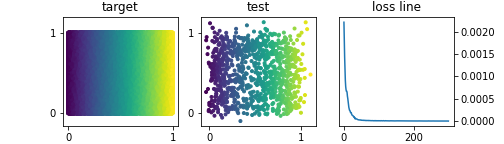
\includegraphics[width=8.5cm]{f1_0.01_300_1000}}
%  \vspace{2.0cm}
\end{minipage}
%  \vspace{2.0cm}
\begin{minipage}[b]{1\linewidth}
  \centering
  \centerline{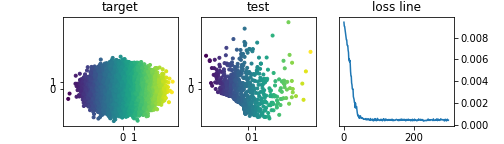
\includegraphics[width=8.5cm]{f2a_0.01_300_1000}}
%  \vspace{2.0cm}
\end{minipage}
%
\caption{$f_1$ and $f_{2a}: L2 = 1e^{-2}$}
\label{fig:res}
%
\end{figure}

When $L2 = 0.01$, the $f_1$ network trains well, with good spread of data, mostly contained within the bounds of 0 and 1.  The $f_{2a}$ network doesn't learn so well, the input data forming a two orthogonal, normal distributions, but the test output fails to train so well, with strong centralisation of data and a general tendency towards positive values.

\begin{figure}[htb]
\begin{minipage}[b]{1\linewidth}
  \centering
  \centerline{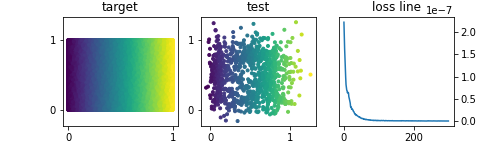
\includegraphics[width=8.5cm]{f1_1e-06_300_1000}}
%  \vspace{1.5cm}
\end{minipage}
%
\begin{minipage}[b]{1\linewidth}
  \centering
  \centerline{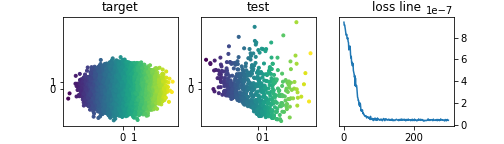
\includegraphics[width=8.5cm]{f2a_1e-06_300_1000}}
%  \vspace{1.5cm}
\end{minipage}
%
\caption{$f_1$ and $f_{2a}$, $L2 = 1e^{-6}$}
\label{fig:res}
%
\end{figure}

When $L2 = 1e^{-6}$, the $f_1$ network again trains well, with good spread of data, mostly contained within the bounds of 0 and 1.  The $f_{2a}$ network doesn't learn so well, the input data forming two orthogonal, normal distributions, but the test output again tends toward positive values.

\begin{figure}[htb]
\begin{minipage}[b]{1\linewidth}
  \centering
  \centerline{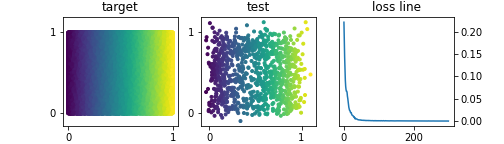
\includegraphics[width=8.5cm]{f1_1_300_1000}}
%  \vspace{1.5cm}
\end{minipage}
%
\begin{minipage}[b]{1\linewidth}
  \centering
  \centerline{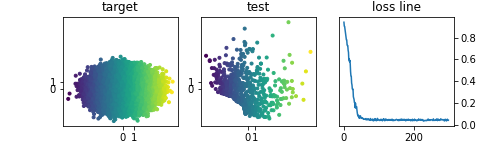
\includegraphics[width=8.5cm]{f2a_1_300_1000}}
%  \vspace{1.5cm}
\end{minipage}
%
\caption{$f_1$ and $f_{2a}$, $L2 = 1$}
\label{fig:res}

\end{figure}
\hfill

When $L2 = 1$, both the $f_1$ and $f_{2a}$ networks both train and deliver similar outputs as with previous levels of L2 regularisation, however, performance is not as good, with loss, predictably 2 orders of magnitude higher than when $L2 = 1e^{-2}$.


% To start a new column (but not a new page) and help balance the last-page
% column length use \vfill\pagebreak.
% -------------------------------------------------------------------------
%\vfill
%\pagebreak

\section{CONCLUSION}
\label{sec:CONC}

Write a conclusion. 

% References should be produced using the bibtex program from suitable
% BiBTeX files (here: strings, refs, manuals). The IEEEbib.bst bibliography
% style file from IEEE produces unsorted bibliography list.
% -------------------------------------------------------------------------

%\vfill\pagebreak

\bibliographystyle{IEEEbib}
\bibliography{refs}

\end{document}
